\documentclass[referee, 
	            sn-basic]
           {sn-jnl}

\usepackage{lineno,hyperref}
\usepackage{longtable, booktabs, amsmath, textcomp}
\usepackage{natbib}

% Put Abstract on new page to create title page as per Oecologia guidelines
	\usepackage{etoolbox}
	\pretocmd{\abstractname}{\newpage}{}{}

% Springer stuff 
\jyear{2022}%
\raggedbottom
\unnumbered% uncomment for unnumbered level heads

\begin{document}
\raggedright

\title[Rangeland grasshoppers and prescribed fire]{Attracted by higher crude protein, grasshopper abundance and offtake increase after prescribed fire\footnote{Author contributions:
NGH collected data. 
NGH and DAM analyzed data. 
NGH wrote the initial draft of the paper, which DAM and CLW edited with input from LV and DB.
LV was responsible for the prescribed fire treatments from which data were collected. 
DB provided grasshopper expertise and sampling equipment. }}


\author*[1]{\fnm{Nicholas Gregory}  \sur{Heimbuch}}\email{ngh11@pitt.edu}

\author[2]{\fnm{Devan Allen} \sur{ McGranahan}}\email{Devan.McGranahan@usda.gov}
\author[3]{\fnm{Carissa L.} \sur{ Wonkka}}\email{Carissa.Wonkka@usda.gov }
\author[2]{\fnm{Lance} \sur{Vermiere}}\email{Lance.Vermiere@usda.gov}
\author[3]{\fnm{David} \sur{ Branson}}\email{David.Branson@usda.gov }

\affil*[1]{\orgname{University of Pittsburg}, 
	     \orgdiv{ },
              \orgaddress{\street{ }, 
            		     \city{Pittsburg},
            		     \postcode{ }, 
           		     \state{Pennsylvania},
            		     \country{USA}}}

\affil[2]{\orgname{USDA Agricultural Research Service}, 
	     \orgdiv{Livestock \& Range Research Laboratory},
              \orgaddress{\street{243 Ft. Keogh Rd.}, 
            		     \city{Miles City},
            		     \postcode{59301}, 
           		     \state{Montana},
            		     \country{USA}}}
\affil[3]{\orgname{USDA Agricultural Research Service}, 
	     \orgdiv{Northern Plains Agricultural Research Laboratory},
              \orgaddress{\street{1500 N Central Ave}, 
            		     \city{Sidney},
            		     \postcode{59270}, 
           		     \state{Montana},
            		     \country{USA}}}
        

           		     
\clearpage

\abstract{Little research has been done to examine the influences of fire and drought on grasshopper herbivory patterns. 
Climate warming is producing more frequent and more intense droughts in the Northern Great Plains region of the United States, affecting herbivore resource availability and stressing the range ecosystem. 
This study created three different time since fire treatments to examine how indirect fire effects (improved forage quality) affect the density and offtake of local grasshoppers.
Both offtake and density were significantly higher in burned locations compared to unburned control plots. 
Burned plot grasshopper density increased greatly over time, while density remained constant in unburned locations. 
These density patterns appear to be the direct result of the high protein content found in burned locations. 
The results raise further questions into the mechanism that produces the magnet effect in range grasshoppers. 
These results also highlight the importance of understanding how fire will interact with future climate conditions to affect range herbivore interactions.} 
\keywords{prescribed fire; }

\maketitle
\begin{linenumbers}

\section{Introduction}

With global climate continuing to warm, rangeland herbivores must adapt
to flaring environmental disturbances. Drought and fire are among the
most prevalent disturbances occurring in the American Midwest. As
anthropogenic climate change continues to shift weather patterns,
rainfall in the northern Great Plains is predicted to increase in the
spring and fall, with annual droughts developing through summer months
\citep{derner2018}. Aboveground net primary productivity (ANPP) in
grassland ecosystems is severely reduced by drought conditions
\citep{hoover2014}. Legacy effects from these droughted summers are not
clearly understood on long timescales, giving range herbivores variable
forage availability in the years to come \citep{hoover2014}.

As droughts continue to worsen in summer months, fire will become even
more frequent in range ecosystems \citep{donovan2017, donovan2020}. In
fact, mean wildfire frequency more than tripled from 2005-2014 compared
to the previous 9 year mean \citep{donovan2017}. Despite the ANPP
reduction, patch burning treatments are able to buffer the drought
losses through improved forage protein content \citep{spiess2020}. Fire
produces a spike in crude protein, the benchmark measurement for forage
quality, which then decreases over time \citep{allred2011}. Even in
homogeneous fire regimes, fire still improves protein content and
removes accumulated grass detritus, however it can also weaken the
biodiversity of the region, creating inconsistent annual forage
production \citep{mcgranahan2016}.

The effects of these disturbances on rangeland ungulates are well
understood. Drought reduces plant biomass and leads to an exodus of
herbivores out of the droughted location and into wetter, more
productive environments \citep{trisos2021}. Due to lowered productivity,
livestock who are unable to leave the droughted rangeland experience
reduced weight gain \citep{allred2014}. On burned rangeland, ungulate
species follow a pyric herbivory feeding pattern, spending more time
grazing in burned patches compared to unburned pasture
\citep{fuhlendorf2009, parrini2010}.

Grasshopper response to fire and drought, on the other hand, still has
many open ended questions. Drought depresses reproductive fitness of
grasshoppers remaining in warm, droughted locations compared to
grasshoppers in undroughted locations \citep{rosenblatt2018}. Fire's
relationship with herbivorous insect species is more complicated. Large
fires can easily kill adult grasshoppers and destroy eggs laid in
shallow soil \citep{branson2013}. Whether grasshoppers experience the
same improved growth that livestock experience from burning treatments
is still the subject of ongoing research. Grasshoppers prefer high
nitrogen content forage to spur growth and development and improve
fecundity \citep{schmitz2010}. While feeding on plants, grasshoppers are
able to monitor their protein and carbohydrate intake to maintain ideal
nutrient ratios \citep{behmer2009, behmer2008}. For instance,
grasshoppers will choose to forage on plants high in carbon content to
increase metabolism and respiratory function \citep{schmitz2010}. More
research is required to understand whether a low nutrient, droughted
range ecosystem will produce the same magnet effect on grasshoppers that
draws ungulates to recently burned prairie.

Our goal for this study is to examine how small-scale fall and spring
burns indirectly affect grasshopper herbivory on a droughted mixed grass
prairie. The primary indirect effect examined in this study is the
improved forage quality produced after fire events \citep{allred2011}.
Previous research into fire's effect on grasshopper density have been
conducted on relatively large burn areas
\citep{branson2005, vermeire2004}. Thus, it is currently unclear how
grasshoppers react to and utilize small patches of heightened resource
quality within a low quality, droughted landscape. The summer of 2021
was incredibly dry in eastern Montana, producing the necessary droughted
forage conditions for us to examine this research question.

\hypertarget{methods}{%
\section{Methods}\label{methods}}

Our study was conducted on a research range operated by the Fort Keogh
livestock and range research laboratory in Miles City Montana. This
mixed grass prairie research location is dominated by western wheatgrass
(Pascopyrum smithii) and, during the summer of 2021, the migratory
grasshopper (Melanoplus sanguinipes). These grasshoppers are frequently
responsible for the largest outbreaks, making the migratory grasshopper
especially damaging to farmers and ranchers throughout the Great Plains
\citep{onsager2000, olfert2021}. We selected nine, 375
m\textsuperscript{2} plots to test three different time-since-fire
treatments with three repetitions each: a fall burn treatment, a spring
burn treatment, and an unburned control treatment. These plots were
situated in a large ungrazed pasture with a two meter buffer zone
between plots.

\hypertarget{offtake}{%
\subsection{Offtake}\label{offtake}}

We identified 2 exclosure and 2 control sites on each of the 9 different
plots with vegetation that reflected the overall grass assemblage of the
plot. We erected one, 0.25 m\textsuperscript{2} exclosure on July 1st,
and a second exclosure and two control structures of the same area on
July 7th. This gap in construction was to ensure that our exclosures
were successful in keeping the grasshoppers out and to gather the
equipment for the other structures. Similar to previous grasshopper
herbivory studies, our exclosures consisted of a PVC pipe skeleton with
heavy nylon netting which kept grasshoppers out of the exclosure area
\citep{parker1985}. The netting created a shading effect that reduced
sunlight intensity by 400 w m\textsuperscript{-2} compared to the
surrounding area. We designed the control structures to remain open on
the north/south faces to allow grasshoppers to enter the study site
while still producing shading conditions matching the exclosures during
peak photosynthesis hours. Our control structures ensured that shade
would not influence grass development and skew our offtake measurements.

I checked every exclosure routinely for grasshopper breaches with no
more than 48 hours elapsing between examinations. The large margin of
error in our spring burn offtake is likely due to an exclosure breach
that occurred on July 19th, 19 days into the experiment timeline. After
a 48 hour break between quality checking the exclosures I noticed a
number of grasshoppers had made it into the exclosure after it sustained
storm damage, so grasshoppers could have been actively foraging in the
exclosure for a maximum of two days. Although this was a short period of
possible contamination, this is the most likely cause for the wide
margin of error. There was no statistical difference in offtake rate
between spring and fall burn treatments. After 40 days, on August 9th, I
clipped and bagged all aboveground biomass within the 0.25
m\textsuperscript{2} test areas for later analysis in the Fort Keogh
range sciences lab. During clipping, I counted and recorded individual
grass tillers in the burn treatment plots to compare data on per tiller
offtake across burn treatments. In the lab, I dried all the grass
biomass samples at 60\(^\circ\)C for two days, so that no moisture
remained, and weighed them to the nearest 0.0001 gram. The difference in
dry weight between exclosures and controls on the same plot provided us
a measure for proportional offtake by grasshoppers between burn
treatments.

\hypertarget{forage-quality}{%
\subsection{Forage Quality}\label{forage-quality}}

On the 26th day of the study period, roughly halfway through the
experiment, I randomly selected 40 tillers of western wheatgrass from
each plot by tossing a marker flag in the air and clipping the
aboveground biomass of the tiller nearest from where it landed. This
collection procedure guaranteed that my sampled tillers were
representative of the plot composition without selection bias. I
returned these tillers to the lab and separated leaves and stems to
assess forage quality differences between the two plant organs. I dried
the stems and leaves and ground them into fine powders which I then
analyzed in a Carbon/Nitrogen analysis machine in the lab. Each plot
produced a diagnostic graph representing the crude protein content of
the analyzed forage.

\hypertarget{density}{%
\subsection{Density}\label{density}}

I assessed grasshopper density on each plot using ring count methodology
\citep{onsager1977, joern2013}. On July 8th, I placed 5 .1 m rings on
each plot in an ``X'' shaped pattern, with each ring approximately 1.5 m
apart. Because our plots were only 375 m\textsuperscript{2} this pattern
kept our rings the correct distance from one another while also
providing buffering space from the plot edges. Between July 9th and
August 6th, I measured abundance on each plot a total of 19 times. For
each count I walked slowly through the plot and agitated the area near
each ring with a long stick and recorded the number of grasshoppers to
leap out from within the ring. All counts were conducted between 1000
and 1200 for consistent solar conditions, and the temperature was
recorded at the beginning of each count.

\hypertarget{data-analysis}{%
\subsection{Data analysis}\label{data-analysis}}

To determine whether accessibility to grasshoppers affected standing crop, we subtracted the dried biomass values of control frames from that of their paired grasshopper exclosure frames (n = 6 observational units per treatment) and found the mean of these two differences for each plot (n = 3 experimental units per treatment). 
We used a linear model with the intercept term removed to test each of the three difference values against 0 (null hypothesis: no difference in standing crop between grasshopper exclosures and control frames) using the \texttt{lm} function in the \textsf{R} statistical environment \citep{Rcore2020}. 
We tested pairwise contrasts in standing crop differences across each treatment with a post-hoc Tukey test using \texttt{TukeyHSD}.

We determined whether crude protein content varied with fire treatment and plant organs (leaves vs. stems) by fitting each term and their interaction in an ANOVA.
Pairwise contrasts among fire treatments were again tested with \texttt{TukeyHSD}.

To determine if there were general linear trends in grasshopper abundance patterns over the course of the study, we conducted a nonparametric test of the Kendall's tau (\(\tau\)) statistic fit to the grasshopper count data within each burn treatment using the \texttt{kendallTrendTest} function in the \emph{EnvStats} package for
\textsf{R} \citep{millard2013}.
To compare the relative rates of change over the study period, we plotted the estimated slope of the trend for each burn treatment and the associated 95\% confidence intervals as returned by \texttt{kendallTrendTest}.

\section{Results}

\begin{figure}
\centering
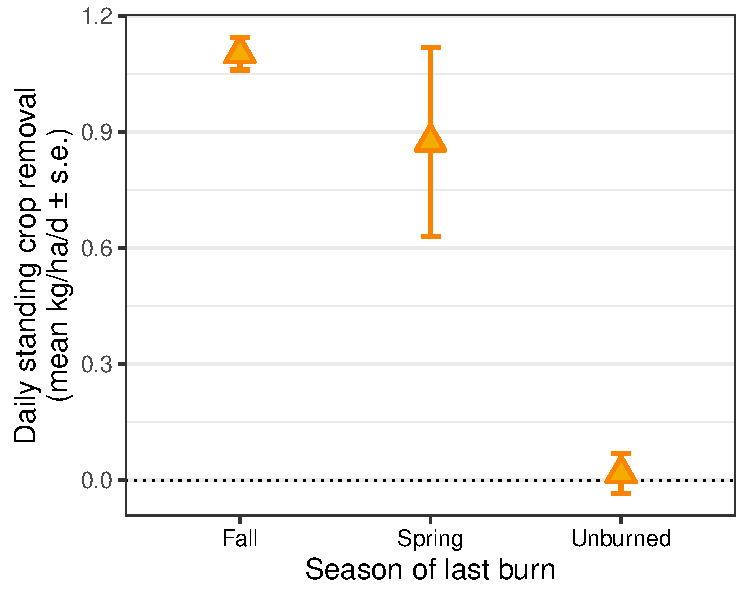
\includegraphics{removal_gg-1.pdf}
\caption{Mean differences in standing crop between grasshopper exclosures and control frames in plots with three different fire treatments. 
Standing crop was determined by clipping at the end of the four-week study period and differences attributable to grasshopper removal are expressed as mean kg per ha per day.}
\label{removal} % Fig.~\ref{removal}
\end{figure}

Standing crop was statistically-significantly lower outside of grasshopper exclosures in both fall and spring burns (\(t =\) -7.6,
\(P\) \textless{} 0.001 and \(t =\) -6, \(P\) \textless{} 0.001, respectively). 
There was no difference in offtake among spring and fall burns (\(P\) \textgreater{} 0.05), with grasshoppers removing approximately 1.0 ($\pm$ 0.2) kg ha\textsuperscript{-1} d\textsuperscript{-1} in each (Fig.~\ref{removal}). 
Standing crop was not different between grasshopper exclosures and areas accessible to grasshoppers in unburned plots (\(t =\) -0.12, \(P\) \textgreater{} 0.05).
 Offtake was significantly lower in unburned plots than plots burned in both the previous fall and spring (\(P\) \textless{} 0.01 and \(P\) = 0.01, respectively).

\begin{figure}
\centering
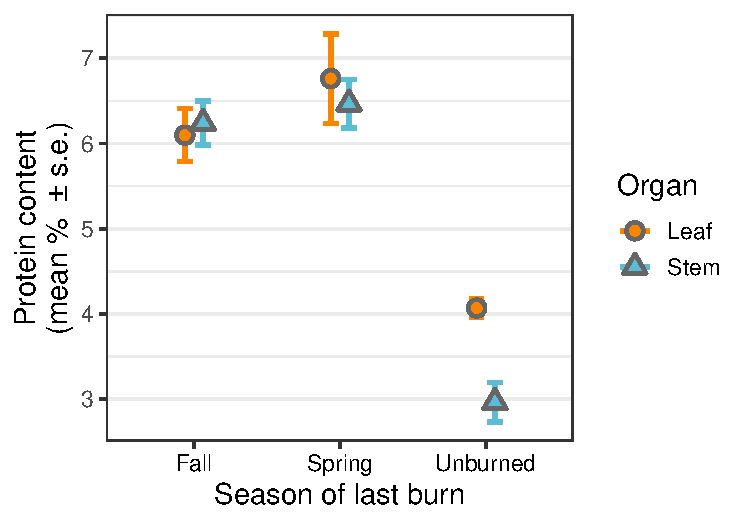
\includegraphics{value_gg-1.pdf}
\caption{Mean protein content of western wheatgrass \emph{Pascopyrum smithii} sampled from three burn treatments as a percentage of total dry matter. 
Red circles indicate the protein content of leaves; blue triangles are stems.}
 \label{value} % (Fig.~\ref{value})
\end{figure}

Crude protein content varied among the fire treatments (\(t =\) 57, \(P\) \textless{} 0.001; (Fig.~\ref{value}). 
Crude protein content in fall and spring burns averaged 6.4\% ± 0.2 s.e. and did not differ among each other (\(P\) \textgreater{} 0.05). 
But crude protein content in unburned  plots was lower than in both fall and spring burns plots (-2.7, \(P\) \textless{} 0.001 and -3.1, \(P\) \textless{} 0.001, respectively).

Across all samples, crude protein content did not vary among leaves and
stems (\(t =\) 2.7, \(P\) \textgreater{} 0.05). Despite a trend towards
higher crude protein in leaf tissue in unburned plots (Fig.~\ref{value}), the
pattern was not influential enough to create a significant fire
treatment \(\times\) organ interaction (\(t =\) 2.1, \(P\)
\textgreater{} 0.05).

\begin{figure}
\centering
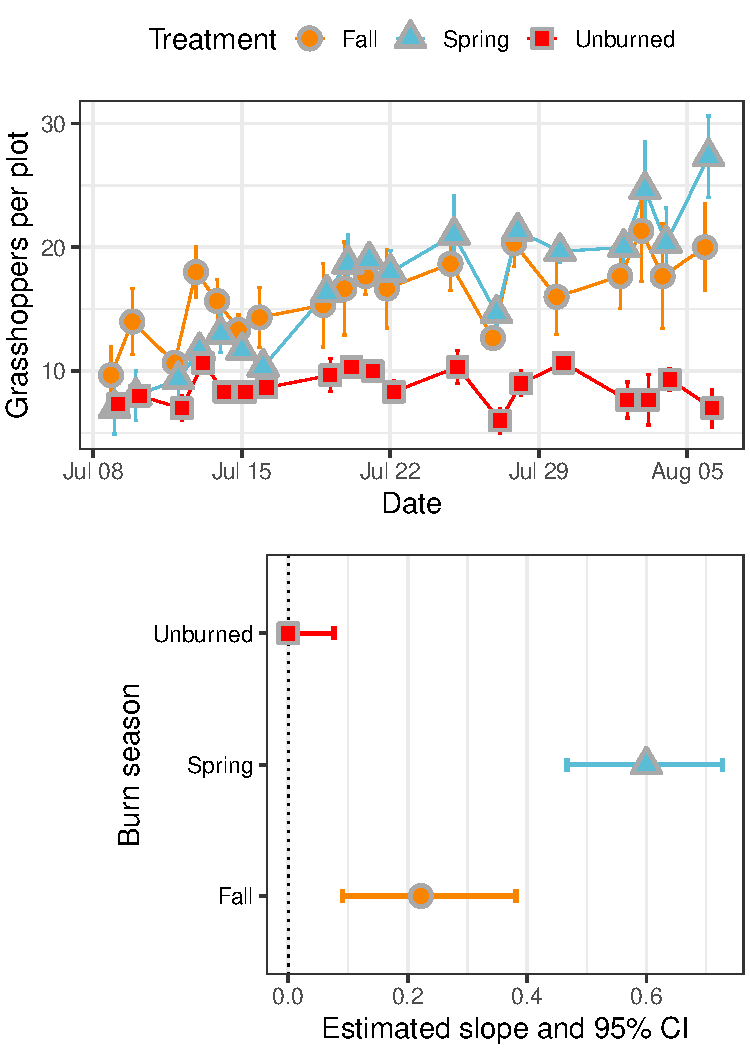
\includegraphics{tau_gg-1.pdf}
\caption{Observed grasshopper counts per square meter. 
Red indicates data taken from fall burn treatments, green from spring burn treatments, and blue from unburned (control) plots.
\emph{Bottom} shows data from Kendall's Tau statistic which assessed the observed count trendline consistency over time. 
Our tau values were compared against the null hypothesis that there was no trend in our data. 
95\% confidence intervals were calculated to show the possible variance in slope for the data over time.}
\label{tau} % Fig.~\ref{tau}
\end{figure}

Grasshopper abundance was similar across plots at the beginning of the study period (early July) but increased significantly over the next month in fall and spring burn plots (\(\tau =\) 0.29, \(P\) \textless{} 0.01 and \(\tau =\) 0.62, \(P\) \textless{} 0.001; Fig.~\ref{tau}). 
Grasshopper abundance remained constant over the study period in unburned plots (\(\tau =\) 0.039, \(P\) \textgreater{} 0.05). 
While grasshopper abundance increased in both burn treatments, the rate of increase was approximately three times greater in plots that had been most recently burned in the spring than those that had been burned in the previous fall (Fig.~\ref{tau}, \emph{bottom}), which represented more than a five-fold increase in density from approximately 10 to 55 grasshoppers m\textsuperscript{-2} (Fig.~\ref{tau}, \emph{top}).

\hypertarget{discussion}{%
\section{Discussion}\label{discussion}}

Previous research indicates that prescribed fire reduces grasshopper
density \citep{joern2004, vermeire2004}, our study, however, saw
heightened density in small patch burning treatments which could have
massive implications for predicting rangeland herbivore competition.
Fire as a method of control varies greatly in effectiveness from species
to species; certain species, such as Hesperotettix viridis, can be
reduced by as much as 88\% \citep{vermeire2004}. Flightless species of
grasshopper and species that are heavily reliant on specific plant hosts
are especially susceptible to fire disturbances \citep{matenaar2014}.
Thanks to nutrient buffering produced by fire treatment
\citep{spiess2020}, protein availability produced a magnet effect which
we believe caused the heightened density and offtake in burned plots
\citep{meyer2002}. These findings indicate fire disturbance can produce
pockets of extreme competition between range herbivores, with much less
forage for ungulates than what is seemingly available.

M. sanguinipes' preferred diet is a nitrogen and carbohydrate ratio of
1:1, making them especially robust and better able to adapt to
nutritionally variable seasons \citep{behmer2008}. Furthermore, these
grasshoppers have the fastest egg production rate at intermediate
dietary nitrogen levels of around 4\% \citep{joern1998} and use nitrogen
to maintain their health and function \citep{schmitz2010}. Due to their
robust qualities, these grasshoppers were incredibly abundant on the
Northern Great Plains in the summer of 2021. Although our burned plots
had higher nitrogen than what is ideal for egg production, the
competition between grasshoppers and the overall low nitrogen content of
the landscape pushed M. sanguinipes to our plots to supplement their
diets. Primary productivity in the Northern Great Plains is directly
linked to rainfall \citep{padbury2002}, therefore the steady increase in
grasshopper density on our burn treatment plots is most likely
attributable to an intensification of the magnet effect as the summer
long drought progressed given that emergence typically peaks in late
June \citep{belovsky1995, humphreys2022}. While other research suggests
that grasshoppers can be attracted to heterogeneous areas for
thermoregulatory microhabitats \citep{joern2013}, the rapid increase in
grasshopper density and the worsening of the drought over the summer
points to a nutrient pull rather than a beneficial microhabitat. High
temperatures, which we experienced consistently throughout the summer
heat wave, weaken M. sanguinipes ability to fight infection
\citep{srygley2022}, further indicating that these grasshoppers are
drawn by nitrogen content and not thermoregulation when shade was nearly
completely absent in the burned plots.

Our study differs from other pyric herbivory studies because it was
conducted with small, clustered areas of burn. Because density increased
so greatly with burn in this study, it indicates a need for further
research into small burn resource utilization by range grasshoppers.
Future directions for our study can examine how grasshopper density
changes with distance from a burn edge for a large burn area. This
information could provide a clearer picture of recolonization effects
created by burn scars combined with magnet effects. Recolonization
presents an avenue for this research to be applied to larger burns in
the Great Plains region, which are becoming more and more common.
Grasshopper density changes could also be further examined through the
offtake rate over time. Further research is needed to see if the offtake
rate increased in burned plots over the duration of the drought. This
would show that offtake is directly related to the quality of the
surrounding forage. Because climate change is intensifying drought
conditions \citep{derner2018}, understanding how offtake will change
will better inform ranching practices to ensure sustainable competition
between grasshoppers and livestock.

Our study has important implications for ranch practices in the Northern
Great Plains. Because prescribed fire is so often used as a forage
buffer for cattle ranching \citep{spiess2020}, it is important to know
how much of the available forage will go to cattle and how much will be
consumed by grasshoppers. Our research already goes against the
population dynamics between grasshoppers and prescribed previously
described \citep{joern2004, vermeire2004}, so it is very likely that
grasshopper abundances are being underestimated when determining how
many cattle can be put out to pasture without overgrazing the landscape.
Furthermore, because the density changed so much over the course of the
study, ranchers must reevaluate the level of competition at the
beginning of the season compared to the end of the season when resources
are even more scarce in a drought.

\backmatter


\bmhead{Acknowledgments}

Thanks bugs

\bmhead{Conflict of Interest} 

The authors declare that they have no conflict of interest.

\bmhead{Funding} 

NGH received salary support from the USDA-ARS Plains Area co-funded internship with matching funds from LARRL and NPARL. 
Cheryl Murphy assisted with N analysis at LARRL and Nichole Davis assisted with grasshopper identification at NPARL. 

\bmhead{Ethics statement} 

This article does not contain any studies with human participants or animals performed by any of the authors. 
 

\bibliography{HopperzBib.bib}

\end{linenumbers}
\end{document}
